\documentclass[twocolumn,11pt]{abst}




% タイトル
\title{長距離飛行するストロー飛行機の製作}

\author{北川鼓太朗(指導教員 伊藤恒平)}

%\urlstyle{rm}

\setcounter{page}{27}
\lhead{}
\chead{}
\rhead{{\sf 17・214}\\{\bf 機械工学科}}
\lfoot{}
%\cfoot{{\sf-\ M-\thepage \ -}}
\cfoot{
 \ifnum \value{page} < 10
  {\sf-\ M-0\thepage \ -}
 \else%
  {\sf-\ M-\thepage \ -}
 \fi%
}
\rfoot{}
\renewcommand{\headrulewidth}{3pt}
%\renewcommand{\footrulewidth}{1pt}



\begin{document}
%\layout
\maketitle
\thispagestyle{fancy}
\pagestyle{fancy}

\setlength{\baselineskip}{5.6truemm}
\kanjiskip=.07zw plus 3pt minus 3pt
\xkanjiskip=.07zw plus 3pt minus 3pt


% 本文

\section{はじめに}
\subsection{研究の背景}
当研究室では飛行ロボットコンテストに出場し予選を突破し決勝で結果を残す事を目標としている.そのため飛行機の原理や仕組みといった構造をメインに研究を行っている.今年度も自作の飛行機で大会に出場したが予選敗退となった.敗退の要因であった縦安定についてストロー飛行機製作を通して学ぼうと考えた.

\subsection{研究の目的}
前期は飛行ロボットコンテストのためにレーザ加工などを行っていたが、大会には出場出来たものの決勝には進出することが出来ず予選敗退だった.
しかし大会出場時は飛行機の構成や原理など分かっていなかったため大会後、飛行機を設計するために知っておかないといけない構成や原理を理解するために簡単な飛行機を作り飛行機が飛行出来る原理の勉強を行いたいと考えていた.
胴体は全長:180[mm]、直径を5[mm]のストローを使い、翼の形状、重心位置の関係の勉強を行った長い距離飛ぶ事が出来る飛行機を製作することを目的としている.

\section{ストロー飛行機のモデル}
ストロー飛行機を制作するにあたりモデルの選定をした所,より滑空能力が優れている戦闘機をモデルにすることにした.その中でも日本の代表的な零戦とアメリカ海軍のグラマンを選出した.二機の特徴を下記に記す.

\subsection{零戦}
零戦とは零式艦上戦闘機の略称であり、第二次世界大戦の時日本海軍の戦闘機として活躍していた.太平洋戦争初期の頃は世界最高水準の戦闘機で航続距離が長く、軽快で運動性能に富んでいた戦闘機である.零戦の写真を図\ref{fig:zerosen}に示す.


\subsection{グラマン}
アメリカの航空機会社であるグラマン社が製造した第二次大戦中アメリカ海軍の主力戦闘機である.良好な運動性能、急降下性能を有していたため日本の航空戦力を撃破するのに最も貢献した機体である.グラマンの写真を図\ref{fig:guraman}に示す.

\begin{figure}[htbp]
  \begin{center}
    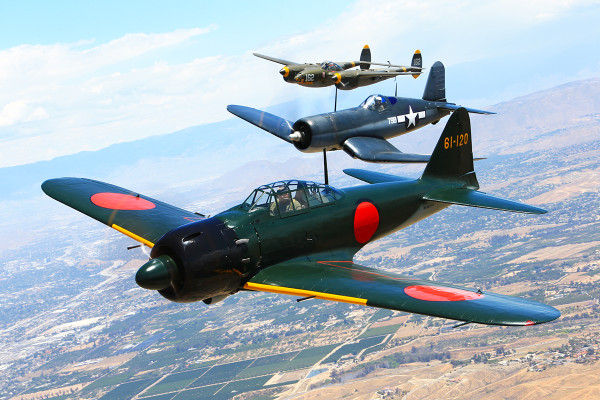
\includegraphics[width=45mm]{zerosen.jpg}
    \end{center}
  \caption{零戦}
 \label{fig:zerosen}
\end{figure}

\begin{figure}[htbp]
  \begin{center}
    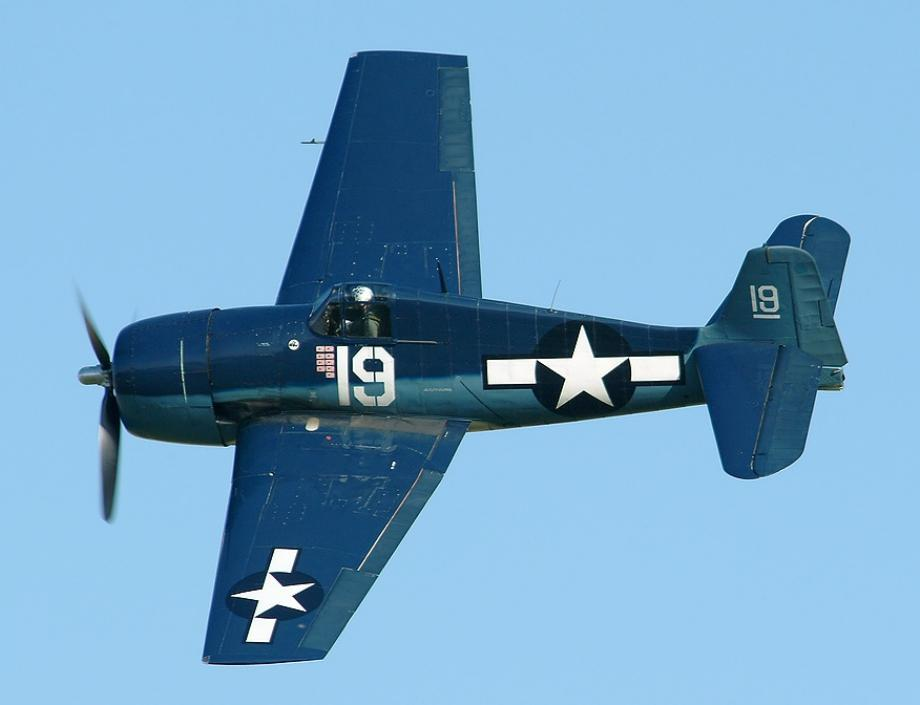
\includegraphics[width=45mm]{guraman.jpg}
    \end{center}
  \caption{グラマン}
 \label{fig:guraman}
\end{figure}

\section{ストロー}

\subsection{ストロー落とし}
本実験は高さ1.5[m]の位置からストローを落とし落下時間を計測する.本実験の目的はストローの空気抵抗を知る事である.

\subsection{ストロー飛ばし}
本実験はある一定の高さからストローを投げ落ちた所までの飛行距離を計測する.本実験の目的はストロー単体の飛行性能を知る事である.

\subsection{零戦の翼のモデル}
零戦のモデルの図面を参考にCAD上で作成した零戦の主翼を図\ref{fig:mainwing}に示す.また零戦の尾翼、垂直尾翼を図\ref{fig:tail}に示す.

\begin{figure}[htbp]
  \begin{center}
    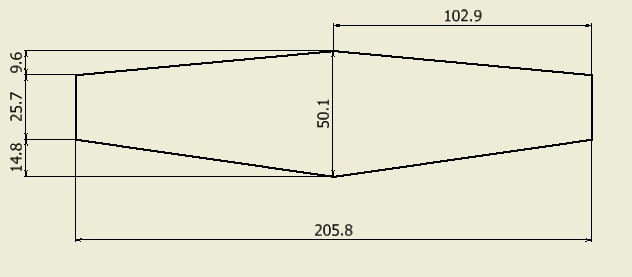
\includegraphics[width=45mm]{mainwing.jpg}
    \end{center}
  \caption{零戦 主翼}
 \label{fig:mainwing}
\end{figure}

\begin{figure}[htbp]
  \begin{center}
    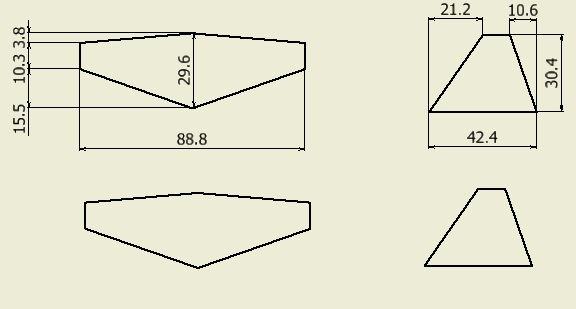
\includegraphics[width=45mm]{tail.jpg}
    \end{center}
  \caption{零戦 尾翼、垂直尾翼}
 \label{fig:tail}
\end{figure}


\subsection{グラマンの翼のモデル}
グラマンのモデルの図面を参考にCAD上でグラマンの主翼を図\ref{fig:guramanmainwing}に示す.またグラマンの尾翼と垂直尾翼を図\ref{fig:guramantail}に示す.


\begin{figure}[htbp]
  \begin{center}
    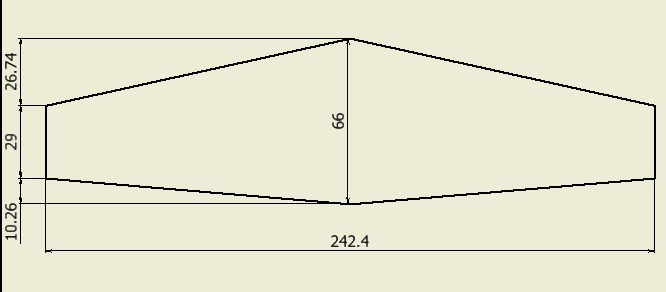
\includegraphics[width=45mm]{guramanmainwing.jpg}
    \end{center}
  \caption{グラマン 主翼}
 \label{fig:guramanmainwing}
\end{figure}

\begin{figure}[htbp]
  \begin{center}
    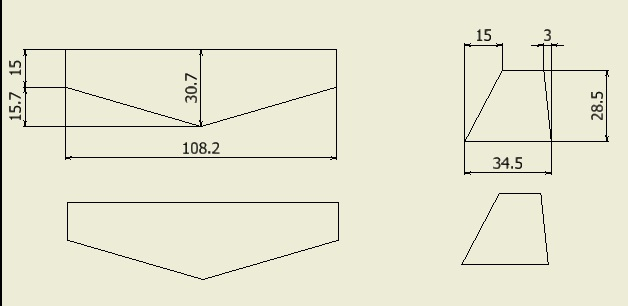
\includegraphics[width=45mm]{guramantail.jpg}
    \end{center}
  \caption{グラマン 尾翼、垂直尾翼}
 \label{fig:guramantail}
\end{figure}

\section{製作方法}
\subsection{レーザ加工}
CAD上で作った翼を製作するためにレーザ加工を用いる.オートフォーカスを用いた場合、スピード:5.0,レーザパワー:17.0が最適な数字であると分かった.この数値で加工を行うと断面が焦げず、綺麗な加工断面を得る事が出来る.またレーザ加工を用いる事でカッターで加工を行うより加工効率が良いため作業の効率化が測れる.

\subsection{接着方法}
もともと翼を一枚のみで製作していたが、壁などに衝突すると翼が折れたりするなど耐久力がなかったため翼を二枚貼り合わせて強度を上げることにした.そこで翼を貼り合わせるための方法を考えた。
候補として、スティックのり・瞬間接着剤・スコッチの強力接着剤・木工用ボンドがあげられた。
まずスティックのりは手に入りやすいが、強度が弱くすぐはがれる.瞬間接着剤・スコッチの強力接着剤の両方とも強度はとてもよいが貼り合わせた瞬間接着されるためズレが生じたときやり直せない不具合が生じた.最後に木工用ボンドは張り付くまで時間がかかるが、手で伸ばす事が出来るため全体をムラなく塗る事が出来た.

\section{飛行試験}

\subsection{重心位置と空力中心の関係}
機体が完成後飛行試験を行った.空力中心と重心位置の関係を変更した場合,飛行距離に違いが出るか実験を用いて調べた.位置関係を変更する方法は機体の先端についている重りを変更する事で位置関係を変えることが出来る.この方法を用いて空力中心が重心位置と比べて前の場合・後の場合・同じ場合と三種類試した.

\subsection{空力中心が重心位置より前の結果}
飛行試験の結果,空力中心が重心位置より前にある場合は宙返りする・機体が頭上げの動作を行う事が分かった.

\subsection{空力中心が重心位置よりも後の場合}
次に空力中心が重心位置よりも後にある場合は飛ばした瞬間失速する・機体が頭下げの動作を行う事が分かった.

\subsection{空力中心と重心位置が同じ位置の場合}
最後に空力中心が重心位置と同じ位置にある場合は頭上げ下げの動作を行わない・機体が真っすぐ飛ぶ事が分かった.


\section{おわりに}
機体に応じて飛行性能に違いがある事が分かった.しかしテーパ翼しか行っていないため矩形翼など他の機体との飛行性能の違いを検証したいと考えている.

% 参考文献
\begin{thebibliography}{8}
\bibitem{sei} 牧野光雄,航空力学の基礎,産業図書株式会社,2016\slash{}07\slash{}15
\end{thebibliography}


\end{document}